\chapter{Fundamentals} % Main chapter title
\label{chap:fund}

% Hier muss alles rein was benötigt wird um die Arbeit zu verstehen.
%   Man kann ja sicherlich grundlegendes Verständis von Recherstrukturen und Organisation vorraussetzten
%   Was also sollte definitiv nochmal erklärt werden?
%
%   - Virtual Memory -> Und vor allem die Kosten, das ist ja auch irgendwo der Aufhänger
%           Der Satz, "tlb is on the critical path of everything really" sollte irgendwann mal kommen
%   - Motivation für vm
%   - Organisationsstrukturen auch im vergleich -> Fazit: Page Tables sind überall und werden tiefer -> vor allem wegeb backwards compatiblity?
%   - Hardware Strukturen für VM - MMU, TLB
%   - Operating system and VM -> Implemented by OS but fixed structures given by MMU
%   -> Problem, fehlende flexibilität ->  A look at several ...
%   -> source: Architectural and operating system support for virtual memory
%   source: issues of implementation

% -------------------------------------------------------------------------------------------------
% A little bit of history?? -> [Denning VM '96] -> Altas
% -------------------------------------------------------------------------------------------------

% -------------------------------------------------------------------------------------------------
%                                           VIRTUAL MEMORY
% -------------------------------------------------------------------------------------------------

This chapter introduces some essential concepts and mechanism which form the basis of the following
chapters. It first gives an overview of \textit{Virtual Memory}, its core requirements,
tradeoffs and implementations.\\
Then the hardware components and caches used to accelerate \textit[Virtual Memory] systems are
presented.\\
An overview of purely software-managed systems follows with a comparison of the general trade-offs
between software-managed and hardware-managed \textit{Virtual Memory} systems.\\
Finally, some specifics of the memory system of the chosen implementation platform, \textit{RISC-V},
are shown.

\section{Virtual Memory}
\textit{Virtual Memory} was first introduced in the Atlas System \cite{fotheringham1961dynamic} to
automate the task of swapping pages between main and secondary memory.
The idea was to make the programms completely unaware of of the real, physical memory by providing
an abstraction layer called virtual memory \cite{denning1996virtual}.\\
With virtual memory, programs appear to have the whole memory space of the machine at their disposal (flexibility) and
nobody to share it with (isolation).\\
The task of managing a programs memory, no matter where in its virtual address space it is, and putting it somewhere
in physical memory now falls to the operating system \cite{denning1970virtual}.\\
This was not only a nice-to-have, but a necessity. The size of programs was increasing faster than the size of main
memory did; while single programs
still fit in memory, operating systems allowed running multiple programs at once, collectively exceeding
the available physical memory \cite{tanenbaumOS}.
% -------------------------------------------------------------------------------------------------

\subsection{Virtual and physical addresses}
The terms of \textit{Virtual} and \textit{Physical} addresses will be coming up a lot in the course of this paper.
Virtual addresses refer to the addresses that are used by the program to reference memory object in its address
space. They are only valid in the programs own address space and may thus be reused by different programs.
Virtual addresses are translated to physical addresses, which are actual addresses to memory locations
on main memory. The \textit{Virtual Memory System} is tasked with performing this translation, creating mappings
and keeping book of those mappings.
\\
Some memory systems using an inverted page tables also use the notion of \textit{effective} addresses.
These form an addition layer of indirection that allows the sharing of pages \cite{jacob1998virtualissues}.\\
Effective addresses will not be discussed here any further.
% -------------------------------------------------------------------------------------------------

\subsection{Memory System Requirements}
In modern systems, \textit{Virtual Memory} does a lot more than swapping pages between main memory and secondary
storage. It is the foundation for a number of requirements to the memory system that are taken for granted
\cite{jacobSoftwaremanagedAddressTranslation1997}.\\
These requirements are as follows:

% -------------------------------------------------------------------------------------------------

\paragraph{Address Space Protection / Isolation} It should not be possible for one process to access the data
of another process, unless explicitly shared.
\cite{jacobVirtualMemoryContemporary1998}

% -------------------------------------------------------------------------------------------------

\paragraph{Shared Memory} Sharing memory allows programms to work on the same physical data with potentially
differing virtual addresses.
\cite{jacobVirtualMemoryContemporary1998}

\begin{marginfigure}
    \includegraphics*[width=1\marginparwidth]{figures/fund_share.pdf}
    \caption{\textbf{Page Sharing}}
\end{marginfigure}

% -------------------------------------------------------------------------------------------------

\paragraph{Large Address Spaces} Programs tend to require more and more memory. Swapping pages can help
to support programs bigger than the actual size of main memory \cite{tanenbaumOS}, but programs may
also require more memory than the theoretical limit set by hardware and software. Modern architectures
use bigger addresses to support programs that require a lot of memory \cite{jacobSoftwaremanagedAddressTranslation1997, jacobVirtualMemoryContemporary1998}.

\todo{pages already definied?}
% -------------------------------------------------------------------------------------------------

\paragraph{Fine-grained Protection} From a security perspective, it is often not desirable to allow the code segment
of a program to be writeable and the data section to be exectuable. \textit{Virtual Memory Systems} provide read-only,
read-write and exectue-only protection on a page granularity\cite{jacobSoftwaremanagedAddressTranslation1997}.
Illegal references may trigger exceptions, which allow the operating system to deal with the program \cite{jacobVirtualMemoryContemporary1998}.

\todo{more on tlb reach in HW section}
% -------------------------------------------------------------------------------------------------

\paragraph{Superpages}
Structures may be bigger than a single page and may thus occupy multiple entries of the translation caches while
only refering to one object. To avoid displacing other caches entries, \textit{Virtual Memory Systems} use
superpages to provide space for bigger objects to increase the reach of cache entries \cite{jacobSoftwaremanagedAddressTranslation1997}.

% -------------------------------------------------------------------------------------------------

\paragraph{Flexibility} Programmers should not have to think about the management
of the resources it requires to do its job, that is the ooperating systems job
\cite{tanenbaumOS}. As such, it should be possible to place the programs code
and data anywhere in the programs virtual address space to make the programmers
job as easy as possible
\cite{jacob1998virtualissues}. % Simplification of the programmes job

\begin{marginfigure}
    \includegraphics*[width=0.9\marginparwidth]{figures/fund_flexibility.pdf}
    \caption{\textbf{Flexibility} Program segments can be dispersed anywhere
        around the virtual address space; the Virtual Memory System has to place
        the pages into actual physical memory.}
\end{marginfigure}
% -------------------------------------------------------------------------------------------------

\paragraph{Sparsity} Big addresses and fine granularity result in a huge address
space with a sparse population for programs that do not require a lot of pages
\cite{tanenbaumOS}.

\begin{marginfigure}
    \centering
    \includegraphics*[width=0.5\marginparwidth]{figures/fund_sparsity.pdf}
    \caption{\textbf{Sparsity / Large Address Spaces} Virtual Memory Systems need to efficiently
        realize huge address spaces with only a few pages being used.}
\end{marginfigure}

% -------------------------------------------------------------------------------------------------

% \paragraph{Memory Mapped IO}
% \cite{tanenbaumOS}

Durch das immer weiter Auseinanderdriften der CPU und Memory geschwindigkeiten und vor allem
durch das größer werden von Addressräumen (von 32 auf 64 bit!) \todo{cite} sind die Ansprüche an
das Virtual Memory system gewachsen und so mussten sich auch die Implementationen weiterentwickeln.

% VM Properties and benefits: Was für Nutzen hat VM?
% Fazit: VM hat sehr nützliche Eigenschaften
% More: jacob1998virtualissues

% -------------------------------------------------------------------------------------------------
%                                IMPLEMENTATION OF VIRTUAL MEMORY
% -------------------------------------------------------------------------------------------------

% Wie können wir VM realisieren? -> Verschiedene Implementationen, Aber hier nicht auf die HW eingehen
%   [ A look at several...]
%   [ Issues of implementation]
\subsection{Implementation of Virtual Memory}
Every virtual memory system has to realize a mapping from virtual addresses of each processes
private, virtual address space to physical addresses that index data in main memory.
This section will provide an overview of how most commonly used virtual memory implementation.\\

% Naive approache
The naive approache is to simply have a big array in main memory. This array can be indexed
using the virtual addresses, at which the physical address to that virtual address is placed.\\
In a 32 bit address space with 4 KB pages, this requires 20 bits per page table entry. This
adds up to \[ 20 * 2^{20} bit = 20971520 / 8 Byte = 2.5 MB \].
To properly isolate the processes from each other, every process needs to have one of those arrays.
To realize fine-grained protection of pages, there would also need to be some bits per array entry
for read/write/execute rights.\\
With 64 bit computer, the space requirements for such page tables would be even higher.

\subsubsection{Hierarchical page tables}
\todo{Verschiedene andere namen -> aus den übersichtspapern [a look at several, issues of impl], radix tree}
Um die Speicherkosten der Verwaltung der Pages zu reduzieren benutzten die meisten \todo{cite?}
Virtual Memory Systeme eine Multi-Level Page Table, oder auch hierarchische Page Table genannt.
Diese ähnelt aber in ihrere Struktur weniger einer Tabelle sondern mehr einem Baum dessen Nodes tabellen
von PTEs sind.
Hier wird die Virtuelle Page nummer nochmal in mehrere Teile unterteilt. Jeder Teil der VPN
wird benutzt um eine kleiner Tabelle zu indizieren. Der indizierte PTE verweißt dann auf die
nächste kleinere Page Table, die dann entsprechend mit dem nächsten Teil der VPN indiziert wird.
Je nach implementierung können hier bis zu 5 weitere indirektionen anfallen.
Ein gängiges Schema wie es z.B. in der RISC-V ISA spezifiziert wird ist Sv39, dass insgesamt
3 Level pro Page Table Tree vorsieht\cite{riscvreader}. Dieses Schema is auch nochmal
in Figure \ref{fig:fund:pagetree} zu sehen.
\begin{figure*}[t]
    \centering
    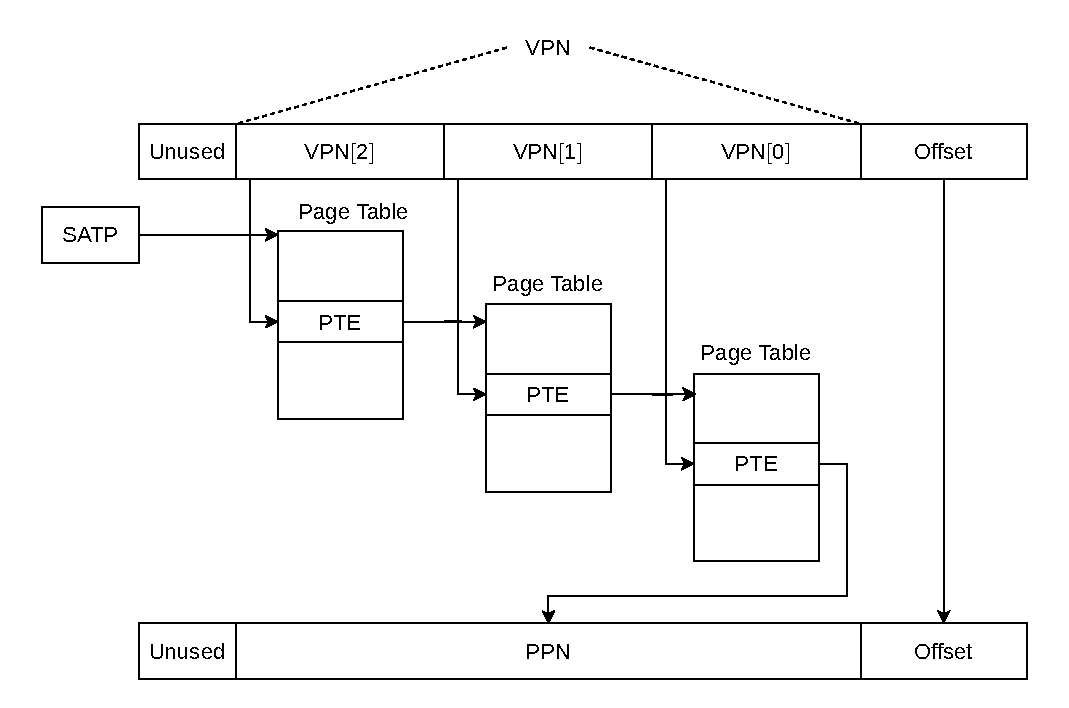
\includegraphics[scale=.8]{figures/VM-Tree.pdf}
    \caption[RISC-V Sv39 3-Level Page Tree]{Three-step page walk with a RISC-V Sv39 Page Table Tree:
        The value in the \texttt{satp} register is the base of the root page table; \texttt{VPN[2]}
        is the index into the root page table; the indexed \texttt{PTE} points to the next page table.
        This traversal continues until the bottom of the page table is reached. The last \texttt{PTE}
        contains the \texttt{PPN} of the physical address which can then be combined with the offset
        bits to make the full physical address}
    \label{fig:fund:pagetree}
\end{figure*}

% Fazit -> Viele Main Memory Zugriffe -> Teuer
Das traversieren der Page Table zum finden des Mappings benötigt pro Level eine weitere Memory reference\todo{cite}
und da das Ermitteln des Mappings auf dem kritischen Pfad jeder Memory-operation befindet,  sodass
es im schlimmsten fall, wenn alle caches missen, zu 5 memory accesses kommen muss (bei einem 5 -level
paging scheme) nur um das Mapping für einen Memory Zugriff zu finden.

% Lösung? Hashed!
\subsubsection{Inverted page tables}
Ein alternatives Paging schema geht von der anderen richtung an das ganze ran und stellt statt einen
Eintrag pro theoretischer virtueller Page einen PTE pro physischem Frame zur Verfügung.
Ein physisches Page Frame ist ein Page-aligneter platz im physischen speicher für eine Page.
Somit ergibt sich die anzahl der physischen Frames durch die Größe des Hauptspeichers geteilt
durch die Page-Größe \todo{Pages schon definiert? Auch die variable größe?}.
Vor allem für 64-bit Addressräume hat das den enormen Vorteil, dass nur so viele Seiten verwaltet
werden müssen die es auch tatsächlich physisch gibt.\\
Das Pagetable design hat noch den Vorteil, dass man im besten Fall deutlich weniger Hauptspeicherzugriffe
benötigt. In dem einfachen Design aus Figure \ref{fig:fund:inverted} kann der entsprechende
Page Table entry schon mit zwei Speicherlookups gefunden werden \cite{skarlatos2020elastic}.

% worst case -> collision count only bound by page frame number
Da allerdings die Page Frame INdizies durch eine Hashfunktion aus der VPN berechnet werden, kann es zu
Hashkollisionen kommen. Da die Länge einer Kollisionskette nicht absehbar ist, ist die maximale
Anzahl der Speicherzugriffe um den richtigen PTE zu finden nur durch die maximale Anzahl der
Page Frames und damit durch die größe des Hauptspeichers beschränkt.

% hierachical -> fixed number of refs (but memory usage)
Hier haben die hierarchieschen multi-level page tables den entscheidenden Vorteil, dass sie immer
die feste Anzahl an Speicherzugriffen benötigen um den PTE zu ermitteln.

% Hash anchor to reduce the collision count
Typische Inverted page table designs haben meistens noch eine sogenannte Hash Anchor Table, die zwischen
dem Output der Hashfunktion und der Page Table liegt. Hat der Hash anchor doppelte größe
der Pagetable, lässt sich die durchschnittliche Collision Chain Length halbieren.
Allerdings wird nun mindestens eine Speicherreferenz in jedem Fall mehr gebraucht \cite{jacob1998virtualissues}.
Alternative inverted page table designes erlauben eine dynamische größenänderung der Tabelle um
Hash Collisionen zu verhindern. Dies ist jedoch sehr teuer und wird in der Regel vermieden \cite{skarlatos2020elastic}.

% Inverted Page Table figure
\begin{figure*}[t]
    \centering
    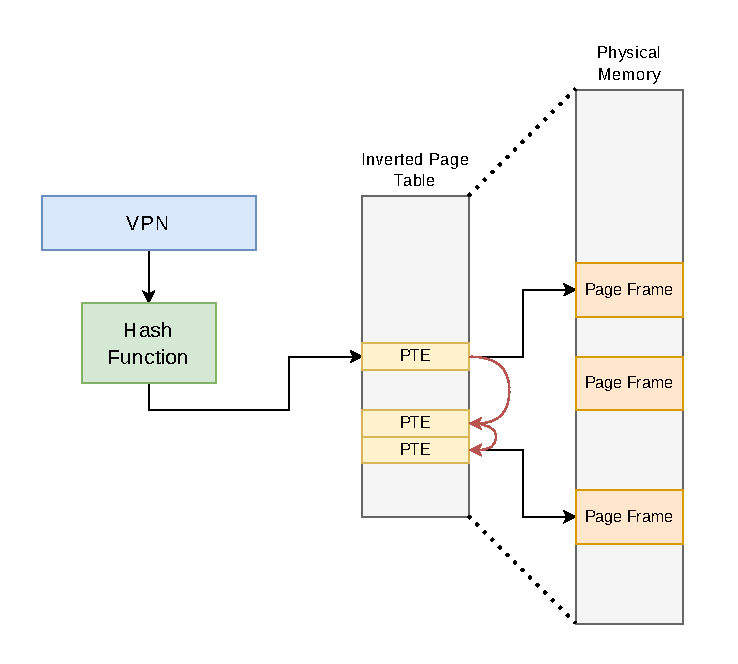
\includegraphics[scale=1]{figures/inverted_pt.pdf}
    \caption[Simple Inverted Page Table Design]{A inverted page table has an entry for every physical
        page frame, reducing memory accesses to a minimum of one. Collisions in the hash table (red arrows) can
        make the access much more expensive. }
    \label{fig:fund:inverted}
\end{figure*}

% Fazit-> Nachteile von Invertierten Page Tables [siehe auch hash dont cache!]
Inverted Page Tables reduzieren zwar die durchschnittliche Zugriffszeit auf die PTEs enorm, sie machen
es jedoch schwerer andere features wie superpages und memory sharing zu unterstützen.
Die Power Architecture unterstützt dies zum Beispiel durch einen zweistufigen übersetzungsprozess\cite{yaniv2016hash}.
% [hash dont cache] -> Hashed paging performs better


% [hash dont cache] -> superpages are harder

% [issues of impl] -> 

% [ A look at several] -> 

% -> Most commonly used in todays hardware -> Multi level page tables
Einen klaren sieger in der debatte hashed vs radix \todo{radix begriff noch einführen} gibt es nicht
und kommerzielle Hardware unterstützt verschiedenste designs die nicht standatisiert sich und z.t.
stark unterscheiden \cite{jacob1998look}.

Moderne INtel prozessoren unterstützen inzwischen radix designs mit einer tiefe von bis zu 5 ebenen,
die nach wie vor 4KB pages benutzten um Kompatibilität zu bewaren.

% Todo, aber größere pages erhöhen tlb reach usw
% Fazit -> Hauptproblem von VM sind teure Hauptspeicherzugriffe im kritischen Pfade von allen Memory Operations

\todo{discussion: Sind die aktuellen VM systeme (vor allem hierachical) noch Zeitgemäß oder nur noch altlast???}
% -------------------------------------------------------------------------------------------------
%                                  END SECTION - VM IMPLEMENTATION
% -------------------------------------------------------------------------------------------------



% -------------------------------------------------------------------------------------------------
%                                            VM HARDWARE
% -------------------------------------------------------------------------------------------------
\cite{denning1970virtual} % Hardware support source
\section{Memory Management Hardware}
Um die Umwandlung der virtuellen in physische Addressen weiter zu beschleuningen nutzen die meisten
modernen Rechner extra hardwarebausteine. Diese bestehen aus einem Hardware Page Table walker (MMU) und
einem Translation Cache, meistens Translation Lookaside Buffer (TLB) genannt\cite{jacobVirtualMemoryContemporary1998}.
% Frage: Besteht das MMU aus TLB + State Walker oder ist MMU der State Walker und TLB einfach extra?
% FIGURE Simple HW Architecture for VM Acceleration Hardware
\begin{figure*}[t]
    \centering
    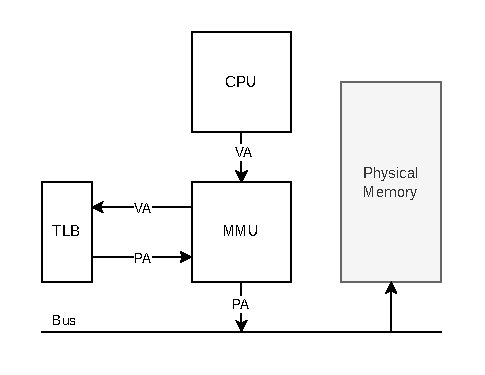
\includegraphics[scale=1.2]{figures/simple_mmu_arch.pdf}
    \caption[A simplified architecture of CPU, MMU and TLB]{A simplified architecture of CPU, MMU and TLB:
        User-level programs running on the \texttt{CPU} try to access main memory with virtual
        addresses; virtual addresses get transparently translated to physical addresses by the
        \texttt{MMU} by either looking up the address in the TLB or by performing a page table
        lookup with the hardware-supported page table design}
    \label{fig:fund:simplearch}
\end{figure*}
% End Figure

% -------------------------------------------------------------------------------------------------

% Davor sollte der Page Table walk bekannt sein
\subsection{MMU}
Das Memory Management Unit (MMU) übernimmt die Aufgabe der addressübersetzung für den Computer.
Dabei steht es zwischen dem Prozessor, der hauptsächlich mit virtuellen Addressen arbeitet und dem
Memory Bus, der mit physischen Adressen zugegriffen wird. Greift der Prozessor auf eine gewisse
virtuelle addresse zu, so führt das MMU einen Page Table walk durch um die zu der virtuellen
Addresse passende physische addresse zu bestimmen. Währenddessen ist der Prozessor effektiv eingefrohren\cite{jacobVirtualMemoryContemporary1998}
\todo{more fine-grained citation? -> Probably not, these are only fundamentals, should however quote overarching works}
\subsection{TLB}
Weil es sehr teuer wäre bei jedem Lade oder Speicher Memory Zugriff einmal die Page Table in hardware zu durchgehen,
gibt es einen Cache für die Übersetzungen, den Translation Lookaside Buffer (TLB). Dieser Cache enthält
most recent Translations von virtueller zu physischer addresse.\\
Das MMU kann also erst mal in den TLB schauen, der parallelisiert und damit extrem schnell durchsucht
werden kann \cite{drepper2007every}.


% Gute quelle für alles hier : [jacob2010memory]
\cite{jacobVirtualMemoryContemporary1998}
% \subsection{A typical Page Table Walk}

% -------------------------------------------------------------------------------------------------
\subsection{PWCs}
\cite{barrTranslationCachingSkip}
\cite{yaniv2016hash}

% -------------------------------------------------------------------------------------------------
\subsection{Address Space Identifies}
% \cite{jacobSoftwaremanagedAddressTranslation1997}
%TODO in the vm requirements , ASIDs are presented as HW-support for address space protection

% -------------------------------------------------------------------------------------------------


% Fazit -> Es gibt hardware strukturen die VM beschleunigen können, die machen es auch schneller
%       ABER: Die machen die VM Software Systeme auch sehr viel rigider und unflexibler
% Kurze Diskussion -> Machen Hardware strukture das wirklich schneller? [ A look at ...]



% -------------------------------------------------------------------------------------------------

% -------------------------------------------------------------------------------------------------

\section{Sofware-based Virtual Memory System}
% VM in Software möglich mit ähnlicher Performance wie hw möglich -> Sollte ja mehr Flexibilität geben
%   [ A look at several...]
% Software managed address translation
% \subsection{Guarded Page Tables}






% -------------------------------------------------------------------------------------------------
% -------------------------------------------------------------------------------------------------
\section{HW VM vs SW VM}
% related work will then come in to discuss approaches close to my approach
% With only software ptw process would have to context switch to the kernel -> Very expensive
% With an MMU the processor essentially just freezes until the memory operation has completed
% \subsection{HW-Dependent PTE Structure} -> inflexibility
Zwischen hardware und software managed translations gibt es einige Erwägungen die in betracht
gezogen werden sollten.

\paragraph{Feste Paging Structuren} Bei Hardware Managed Virtual Memory sind die structuren für
für die Page Tables und Page Table Entries fest von der Microarchitecture definiert.
Dadurch kann das Betriebssystem das Memory Management nicht auf seine zwecke und seinen Use case
zurecht schneiden und ist stuck mit dem fixen design.
Dieses erschwert auch die Portabilität von Systemsoftware, da es keinen Standard für diese
Memory Management Strukturen gibt.
Bei diesen gibt es auch keinerlei standartisierung obwohl es keine bedeutenden Performance unterschiede
in den Verschiedenen designs  gibt \cite{jacob1998look}.

\paragraph{Pipeline freezing / flushing} Bei einem TLB Miss \todo{schon definiert?} kommt es bei
einem hardware verwalteten TLB nur zu einem einfrieren der Pipeline (zumindest für die Instruktionen
die abhängig von dem Speicherzugriff sind). Bei einem software verwalteten TLB wird die Kontrolle
jedoch zurück an das Betriebssystem über eine Exception gegeben, die entsprechend vermerkt,
dass sich die benötigte Adresse nicht im TLB befindet (TLB Miss Exception).
Der Sprung zurück ins Betriebssystem sorgt für einen Context-Switch, es muss also der Zustand
des aktuellen Prozesses gespeichert werden. Dabei wird der Reorder buffer geflushed und die
pipeline massiv gestört. Durch den switch in den Kernel kann es langfristig auch noch zu weiteren
Data und Instruction misses kommen, da ja der Kerneleintritt sicherlich einige Cache lines die der
laufende Prozess benötigt hat überschrieben hat. \todo{Cite}

\paragraph{Embedded} Auch für embedded systems wird es interessanter virtual memory zu nutzen.
Diese würden sicherlich von flexibleren designs profitieren. Außerdem würde die ein Einsparen
an Chipgröße durch weglassen des MMUs auch die Kosten in der Produktion senken. \cite{jacob1998look}
\todo{weiß ja nicht}


% Conclusion of HW vs SW
\cite{jacob1998look} schließt in einer vergleichenden Studie verschiedener HW und SW memory designs,
dass wohl HW basierte Ansätze grundsätzlich performanter sind, aber das SW basierte designs durchaus
viable sind, wenn die caches groß genug sind um die Anzahl der Cache misses zu reduzieren.
Besonders bezüglich der flexibilität haben sw ansätze auch einen großen vorteil, da das VM system
vollständig durch das OS definiert werden kann.
% -------------------------------------------------------------------------------------------------

% -------------------------------------------------------------------------------------------------

% TODO Short discussion hw and sw vm -> common problem: Page Table Walks require in either case a 
% lot of memory references. These costs can be aleviated using caches, but will still cost [ cite a source abouts costs here]

\todo{section on basic operating system structures like exception handler, load store sandwich}

\todo{fundamentals on the implementation platform}
% -------------------------------------------------------------------------------------------------

% -------------------------------------------------------------------------------------------------


\section{RISC-V Basics}
Die Implementation die in dieser Arbeit vorgestellt läuft auf einer RISC-V Platform. Daher ist
es notwendig ein paar Grundlagen zur RISC-V Platform durchzugehen. Relevant sind hier vor allem
das Virtual Memory System, der Exception/Trap Mechanismus und die Control und Status Registers (CSRs), die
die Grundlage der Erweiterung von RISC-V darstellen.
% -------------------------------------------------------------------------------------------------

\subsection{Sv39 Virtual Memory}
\label{fund:sv39}

\todo{explain why the top bits in PTE are all zero (with leichten Bezug zu xv6 impl)}
\begin{figure*}[h!]
    \centering
    \begin{bytefield}[bitwidth=\widefigurewidth/64,bitheight=\widthof{~PBMT~}, bitformatting={\tiny\bfseries}, boxformatting={\centering}]{64}
        \bitheader[endianness=big]{63,62,61,60,54,53,28,27,19,18,10,9,8,7,6,5,4,3,2,1,0} \\
        \bitbox{1}{N} &
        \bitbox{2}{\rotatebox{90}{PBMT}} &
        \bitbox{7}{Reserved} &
        \bitbox{26}{PPN[2]} &
        \bitbox{9}{PPN[1]} &
        \bitbox{9}{PPN[0]} &
        \bitbox{2}{\rotatebox{90}{RSW}} &
        \bitbox{1}{D} &
        \bitbox{1}{A} &
        \bitbox{1}{G} &
        \bitbox{1}{U} &
        \bitbox{1}{X} &
        \bitbox{1}{W} &
        \bitbox{1}{R} &
        \bitbox{1}{V}
    \end{bytefield}
    \caption[RISC-V Sv39 Page Table Entry]{RISC-V Sv39 Page Table Entry}
    \label{fig:theory:sv39pte}
\end{figure*}
% -------------------------------------------------------------------------------------------------

\subsection{Traps}
\todo{Das hier alles in fundamentals?}
% exceptions vs interrupts
Traps sind Teil der RISC-V privilegierten Architecture. Sie bieten einen Mechanismus
um auf externe Events und auf unusual runtime events, also Exceptions, zu reagieren\cite{riscvreader}.
Der Begriff Trap ist ein Überbegriff der nochmal in Interrupts - asynchrone Events - und
Exceptions - synchrone Events - aufgeteilt wird.\\
Besonders von Interesse sind hier die Exceptions, da ein TLB Miss beim ausführen einer Instruktion
passiert, also synchron zur Clock des Prozessors. Allerdings ist es für das Arbeiten mit
dem Qemu und dem xv6 Quellcode auch wichtig die Interrupts mit im Kopf zu behalten, da auf der
einen Seite der Qemu Code exceptions und interrupts in den gleichen Funktionen behandelt und
auf der anderen Seite xv6, bzw. RiscV im allgemeinen einen vereinten Vektor für das handling
von Interrupts und Exceptions nutzt\cite{RISCVInstructionSet}. \\

% Exception registers
Für das Auslößen und Behandeln von Exceptions sind 6 register zentral. Diese gibt es sowohl
für den Supervisor Mode (starting with an s) als auch den Machine Mode (starting with an m).
\todo{priviledge modes schon eingeführt?} Ob für die Exception die machine mode variante des
registers oder die Supervisor Mode Variante verwendet werden sollte hängt von dem Modus ab
in dem die Exception behandelt wird. Im folgenden werden alle Register nur mit dem M-Mode \todo{
    M-Mode als abkürzung für Machine Mode schon eingeführt?
}
prefix dargestellt. \todo{Weil die Exception am ende als M-Mode exception konzipiert wurde?}

% TODO sortierung der Register nach rolle?

% Vector -> mtvec
\textbf{Exception Vector} Der Hart \todo{Begriff Hart schon eingeführt?} bei dem zu einem
außerordentlichen Zustand gekommen ist muss wissen wo die Kernel Routine ist zu der er zur
Exception behandlung springen muss. Dafür enthält \texttt{BASE} field des registers eine
4-Byte alignten physischen Adresse zu der der Program Counter im Exception fall gesetzt wird.\\
Das \texttt{MODE} field erlaut es zwischen einem \texttt{direct} und \texttt{vectored} Mode
umzuschalten. Im \texttt{MODE=Direct} wird bei allen Traps der PC zu BASE gesetzt, bei
\texttt{MODE=Vectored} wird der PC für asynchrone interrupts zu $ BASE+4*CAUSE $ gesetzt.\\
% Delegation -> medeleg

% Data for exception handling -> mcause, mtval, mepc, mscratch
\textbf{Context Information} Um die Exception ordentlich zu behandeln sind einige
Kontextinformationen notwendig. Das \textbf{mcause} Registe enthält den den Exeption Code
der Exception; \textbf{mepc} enthält den Program Counter der Instruktion die zum werfen der
exception geeführt hat; und \textbf{mtval} enthält exception spezifische informationen wie
zum Beispiel die virtuelle Addresse die eine Page Fault Exception ausgelößt hat.
\textbf{mstatus} enthält allgemeine Informationen zum aktuellen Zustand der Hardware.\\

\textbf{Delegation} Normalerweiße werden alle Exceptions im machine mode behandelt, allerdings
kann es manchmal auch sinnvoll sein die die Exception in einem niedrigeren Privilegienmodus
zu behandeln. Mit dem Bitfield im \textbf{medeleg} register kann man für einzelne Exceptions
auswählen, ob diese zum nächst-niedrigeren Privilegienmodus weitergereich werden sollen.\\

% Exception number
\textbf{Exception Code} Jeder exception ist eine eindeutige nummer, der Exception code zugewießen
\cite{riscvreader}. Diese findet sich beim behandeln der Exception im mcause register wieder.

% Zusammenspiel der Register im Exception Fall -> xv6 Book Exception Machinery

\textbf{What the Hardware does} Wenn eine Exception getriggert wird macht die Hardware folgendes:
\begin{enumerate}
    \item Interrupts are disabled by clearing the MIE bit in \textbf{mstatus}
    \item PC is copied to mepc
    \item the current mode is saved to the MPP field in mstatus
    \item mcause is set to the proper exception code
    \item the mode is set to the machine mode
    \item Pc is set to stvec
    \item execution continues at the new pc
\end{enumerate}
% -------------------------------------------------------------------------------------------------

\subsection{Contol and Status Registers}
% Section describing RISC-V CSRs -> Originally in theory
\todo{table of csr space in appendix?}
The RISC-V ISA provides a 12-bit encoding space for 4096 CSRs. A CSR address is logically split
into four parts: The top two bits \texttt{csr[11:10]} specify whether the CSR is read/write or read-only;
\texttt{csr[9:8]} encode the minimum priviledge level that is allowed to access the CSR; \texttt{csr[7:4]}
may be partially used to define a specific use for a range of CSRs. E.g. CSRs with an address
between \texttt{0x7B0} and \texttt{0x7BF} shall be used for Debug-mode-only CSRs. The format
of the CSR addresses is also depicted in figure \ref{fig:theory:csr}.

% RISC-V CSR address bytefield
\begin{figure*}[h!]
    \centering
    \begin{bytefield}[bitwidth={2em}, bitformatting={\bfseries}, boxformatting={\centering}]{12}
        \bitheader[endianness=big]{11,10,9,8,7,4,3,0} \\
        \bitbox{2}{RW/RO} &
        \bitbox{2}{Priv} &
        \bitbox{4}{Usage} &
        \bitbox{4}{Index}
    \end{bytefield}
    \caption[RISC-V CSR address format]{RISC-V CSR address format}
    \label{fig:theory:csr}
\end{figure*}

Each legal CSR address identifies a CSR. The size of the CSRs identified by the CSR address depends
on the values of the SXLEN and UXLEN fields in the \textbf{mstatus} register. Currently, the
specification \cite{RISCVInstructionSet} allows for 32 bit, 64 bit and 128 bit.\\ \todo{disclaimer which we will be using here?}
% Short elaboration on using the csr to write TLB entries -> in the end its on the hardware implementor
RISC-V provides dedicated instructions for read/write and bit manipulation with both register values
and immediates.
\todo{ hardware overhead for writing TLB with CSRs -> future work, is it worth it??}

% What format, how big, how many csrs?
Now with CSRs we have a mechanism to add custom behaviour to the ISA. That answers the ''How?''
of writing TLB entries in software.\\
The next step is to figure out what data is required to create a TLB entry and in what format
this data is best communicated via the CSRs to the computer.\\
% -------------------------------------------------------------------------------------------------






% All approaches are based on a table.
% Überleitung zu meinem Thema -> Avoid all memory references and just have a simple (hash?) function that realizes VM
% [ a look at severeal ] -> conlsion


\begin{figure*}[t]
    \centering
    \begin{bytefield}[bitwidth=\widefigurewidth/56,bitheight=\widthof{~PBMT~}, bitformatting={\tiny\bfseries}, boxformatting={\centering}]{56}
        \bitheader[endianness=big]{55,30,29,21,20,12,11,0} \\
        \bitbox{26}{PPN[2]} &
        \bitbox{9}{PPN[1]} &
        \bitbox{9}{PPN[0]} &
        \bitbox{12}{Page Offset}\\
    \end{bytefield}
    \caption[RISC-V Sv39 Physical Address]{RISC-V Sv39 Physical Address}
    \label{fig:theory:sv39pa}
\end{figure*}


\begin{figure*}[t]
    \centering
    \begin{bytefield}[bitwidth=\widefigurewidth/64,bitheight=\widthof{~PBMT~}, bitformatting={\tiny\bfseries}, boxformatting={\centering}]{64}
        \bitheader[endianness=big]{63,60,59,44,43,0} \\
        \bitbox{4}{Mode} &
        \bitbox{16}{ASID} &
        \bitbox{44}{PPN} \\
    \end{bytefield}
    \caption[RISC-V Sv39 \texttt{satp} CSR]{RISC-V Sv39 \texttt{satp} CSR}
    \label{fig:theory:sv39satp}
\end{figure*}

\begin{figure*}[t]
    \centering
    \begin{bytefield}[bitwidth=\widefigurewidth/39,bitheight=\widthof{~PBMT~}, bitformatting={\tiny\bfseries}, boxformatting={\centering}]{39}
        \bitheader[endianness=big]{38,30,29,21,20,12,11,0} \\
        \bitbox{9}{VPN[2]} &
        \bitbox{9}{VPN[1]} &
        \bitbox{9}{VPN[0]} &
        \bitbox{12}{Page Offset}\\
    \end{bytefield}
    \caption[RISC-V Sv39 Virtual Address]{RISC-V Sv39 Virtual Address}
    \label{fig:theory:sv39va}
\end{figure*}
